\section{Comparando Codificações}
\label{cap:2.5}

Para finalizar este capítulo, é de especial interesse abordar a forma como é feita a comparação entre duas codificações de vídeo diferentes. De forma geral, três valores são capturados durante uma codificação de vídeo: 

\textbf{Taxa de bits por segundo} (do inglês, \textit{bits per second}, bps): representa quantos bits ou kilobits (kb) o \textit{bitstream} gerado possui divididos pelo tempo em segundos do vídeo. Como esse valor é relativo à quantidade de quadros processados, a maioria dos codificadores já fornece esse valor médio.

\textbf{Nível da qualidade da imagem}: indica a diferença objetiva entre a imagem original (pré-codificada) e a imagem decodificada (pós-codificada). Existe, na literatura, uma série de métricas objetivas que capturam a diferença entre as duas imagens, sendo as mais comuns a Relação Sinal-Ruído de Pico (do inglês, \textit{Peak Signal-to-Noise Ratio}, PSNR) \cite{bib:psnr} e a Fusão de Vários Métodos de Avaliação de Vídeo (do inglês, \textit{Video Multi-Method Assessment Fusion}, VMAF) \cite{bib:vmaf}. O valor da métrica PSNR, assim como a taxa de bits, já é fornecido pela maioria dos codificadores após a codificação. Portanto, é a mais usual de ser encontrada na literatura científica, apesar das diversas inconsistências que essa métrica oferece quando comparada com métricas subjetivas ou empregada em vídeos mais complexos, como HDR ou \textit{Screen Content} \cite{bib:mse_wrong}. Note que o cálculo do PSNR é sempre resultante da diferença entre a sequência de vídeo original (âncora) com a versão dessa sequência após a codificação (comparada). Além disso, na transcodificação de vídeos, o PSNR é calculado tendo-se a sequência decodificada como âncora e a sequência re-codificada como comparada.

\textbf{Variação do Tempo de Codificação}: informa a diferença percentual entre o tempo exigido para executar a codificação em observação e o tempo de codificação de referência. Os trabalhos de transcodificação de vídeo apresentados nesta tese visam sempre apresentar um tempo de codificação inferior ao de referência. Portanto, normalmente se apresentam valores de Redução de Tempo (do inglês, \textit{Time Saving}, TS). Para o cálculo da redução do tempo de codificação ou de transcodificação, utilizamos a Equação \ref{eq:7}, onde $Ta$ e $Tb$ são os tempos de codificação original e modificada, respectivamente, e $q$ representa o conjunto de níveis de quantização utilizados.

\begin{equation}
    \label{eq:7}
    TS = 100 * \left ( \frac{1}{n} \sum_{q_0}^{q_n} \frac{Ta_q - Tb_q}{Ta_q} \right )
\end{equation}

É importante destacar que existe uma relação entre a taxa de bits por segundo e o nível da qualidade da imagem, isto é, uma maior quantidade de dados permite armazenar vídeos com maior qualidade de imagem. Ao mesmo tempo, codificadores de vídeo mais modernos são capazes de comprimir vídeos com idêntico nível de qualidade de imagem que outro codificador mais antigo, mas com uma quantidade inferior de dados. Portanto, essa relação entre taxa de bits e qualidade de imagem precisa ser considerada ao se realizar comparações entre diferentes codificadores ou variações de um mesmo codificador. O principal destaque a ser feito é que os níveis de qualidade da imagem também são alterados, o que dificulta a correlação direta nessas comparações.

Dessa forma, \citet{bib:bdrate} desenvolveu uma métrica, denominada Bj{\o}ntegaard Delta(BD)-rate, que relaciona duas codificações diferentes sob a ótica dessas duas variáveis alvo. Para tanto, faz uso do cálculo de uma integral que representa a área entre duas curvas de taxa de bits e nível de qualidade, como apresentado na Figura \ref{fig:9}. Basicamente, o BD-rate equipara os níveis de qualidade e informa a diferença percentual da taxa de bits de uma codificação em relação à codificação de referência. Sendo assim, valores negativos indicam uma redução na taxa de bits, o que é normalmente esperado quando se comparam formatos de codificação de vídeo recentes frente aos mais antigos. Por outro lado, valores positivos de BD-rate indicam um aumento na taxa de bits, o que é mais comum ocorrer nos trabalhos de transcodificação de vídeo acelerado frente aos transcodificadores originais.

\begin{figure}
    \centering
    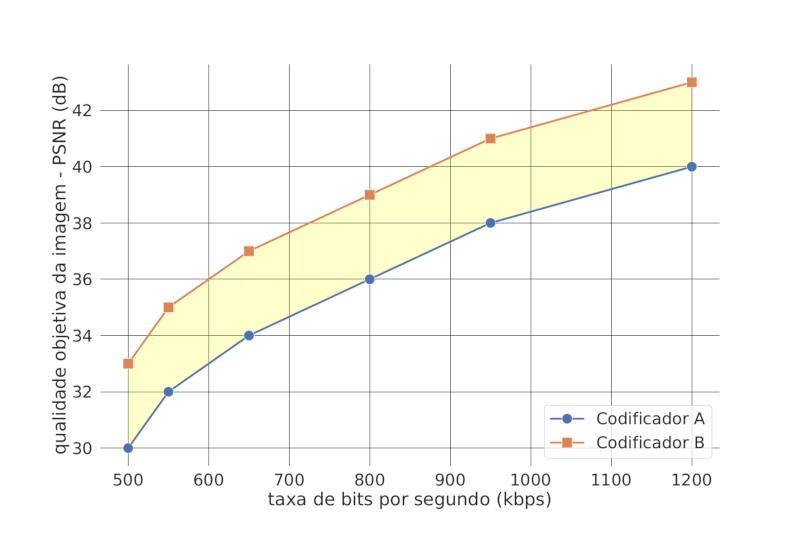
\includegraphics[width=0.85\textwidth]{FIGURES/fig_9.png}
    \caption{Exemplificando duas curvas de BD-rate. Fonte: Elaborada pelo autor.}
    \label{fig:9}
\end{figure}

Finalizamos, então, todos os conceitos básicos necessários para a compreensão do restante desta tese. Para conhecimentos mais aprofundados, recomendamos a leitura das referências bibliográficas apontadas ao longo deste capítulo. No capítulo \ref{cap:3}, apresentamos o estado da arte em transcodificação de vídeo.
